\documentclass[a4paper, 12pt]{article}

\usepackage{multirow}
\usepackage[table,xcdraw]{xcolor}
\usepackage{enumerate}
\usepackage{graphicx}
\usepackage[T5]{fontenc}
\usepackage[utf8]{inputenc}
\usepackage[margin = 2cm]{geometry}
\usepackage{amsfonts, amsmath, amssymb}
\usepackage[none]{hyphenat}
\usepackage{fancyhdr}
\usepackage{float}
\usepackage{hyperref}
\usepackage{caption}
\usepackage[nottoc, notlot, notlof]{tocbibind}

% \captionsetup[table]{skip=5pt}
\pagestyle{fancy}
\fancyhead[L]{Trường Đại học Khoa học Tự nhiên - ĐHQG TP.HCM}
\fancyhead[R]{Nhóm Just $4^{th}$}

\begin{document}

\begin{titlepage}
    \begin{center}
        \vspace*{1cm}
        \Large\textbf{Đại học Quốc gia TP.HCM\\Trường Đại học Khoa học Tự nhiên}\\

        \vfill
        \line(1,0){450}\\[4mm]
        \LARGE\textbf{\MakeUppercase{Classification \& Clustering}}\\[3mm]
        \Large{Khai thác dữ liệu \& Ứng dụng}\\[3mm]
        \Large{Nguyễn Bảo Long - MSSV: 18120201}\\
        \Large{Huỳnh Long Nam - MSSV: 18120212}
        \line(1,0){430}\\
        \vfill

        \vfill
        TP Hồ Chí Minh, ngày 02/12/2020
    \end{center}
\end{titlepage}

\tableofcontents
\thispagestyle{empty}
\clearpage

\section{Thông tin chung}

\begin{enumerate}
    \item Link GitHub: \url{https://github.com/baolongnguyenmac/DataMining-Lab3}
    \item Thông tin thành viên nhóm
    \begin{table}[H]
        \begin{center}
            \begin{tabular}{|c|c|c|c|}
            \hline
            STT & Họ tên          & MSSV     & Email                         \\ \hline
            1   & Nguyễn Bảo Long & 18120201 & 18120201@student.hcmus.edu.vn \\ \hline
            2   & Huỳnh Nam Long  & 18120212 & 18120212@student.hcmus.edu.vn         \\ \hline
            \end{tabular}
            \caption{Bảng thông tin thành viên nhóm}
        \end{center}
    \end{table}

    \item Tỷ lệ tham gia công việc
    \begin{table}[H]
        \begin{center}
            \begin{tabular}{|c|c|l|c|}
            \hline
            STT & Họ tên                    & \multicolumn{1}{c|}{Công việc}     & Tỷ lệ hoàn thành      \\ \hline
            1   & \multirow{4}{*}{18120201} & Tiền xử lý dữ liệu                 & \multirow{4}{*}{50\%} \\ \cline{1-1} \cline{3-3}
            2 &  & Phân lớp dữ liệu bằng Weka Explorer      &  \\ \cline{1-1} \cline{3-3}
            3 &  & Cài đặt và kiểm thử thuật toán K-Means   &  \\ \cline{1-1} \cline{3-3}
            4 &  & Trình bày báo cáo                        &  \\ \hline
            5   & \multirow{3}{*}{18120212} & Phân lớp dữ liệu bằng Experimenter & \multirow{3}{*}{50\%} \\ \cline{1-1} \cline{3-3}
            6 &  & Đánh giá phương pháp phân lớp            &  \\ \cline{1-1} \cline{3-3}
            7 &  & Cài đặt và kiểm thử thuật toán K-Medoids &  \\ \hline
            \end{tabular}
            \caption{Bảng phân chia công việc}
        \end{center}
    \end{table}
\end{enumerate}
\clearpage

\section{Ý tưởng tiền xử lý dữ liệu}

\begin{itemize}
    \item Chi tiết quá trình tiền xử lý dữ liệu được trình bày trong file `Preprocess.ipynb'
    \item Ý tưởng chung
    \begin{itemize}
        \item Xoá các thuộc tính có tỷ lệ thiếu dữ liệu lớn hơn hoặc bằng 50\%
        \item Xoá các dữ liệu dạng IDentification
        \item Điền giá trị thiếu tại các cột có kiểu dữ liệu dạng số bằng giá trị trung bình 
        \item Điều giá trị thiếu cho các cột có kiểu dữ liệu định danh bằng giá trị mode
    \end{itemize}
\end{itemize}
\clearpage

\section{Đánh giá phương pháp phân lớp}

\begin{itemize}
    \item Phương pháp phân lớp nào thường cho kết quả cao nhất?\\
    $\rightarrow$ Theo file "Result.xlsx", khi sắp xếp giảm dần cột "Tỷ lệ mẫu được phân đúng", ta thấy ID3 là thuật toán cho kết quả phân lớp đúng cao nhất (100\%), kế đến là J48 (99.45\%). Nhưng xét tổng quan, với cùng một chiến lược đánh giá, J48 cho kết quả cao và ổn định
    \begin{figure}[H]
        \begin{center}
            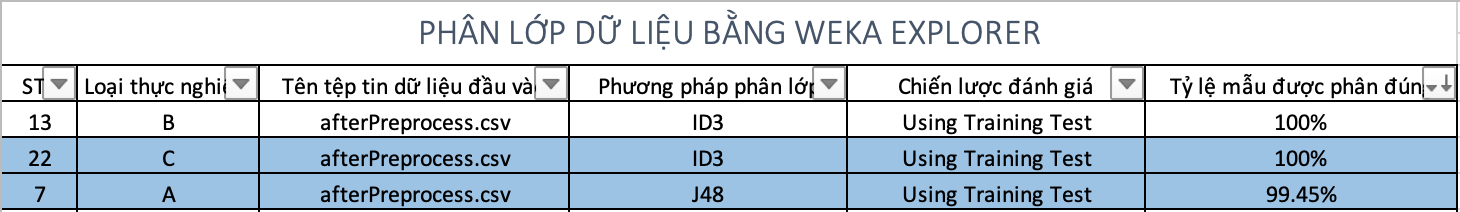
\includegraphics[scale = 0.65]{./img/maxRate.png}
            \caption{Thống kê tỷ lệ mẫu được phân lớp đúng ứng với các thuật toán}
        \end{center}
    \end{figure}

    \item Phương pháp nào không thực hiện tốt và tại sao?\\
    $\rightarrow$ ID3 fit với bộ training test nên độ chính xác khi đánh giá sử dụng bộ training test sẽ cho 100\%\\
    $\rightarrow$ Phương pháp ID3 không thực hiện tốt vì nhược điểm của ID3 là sẽ quá khớp với bộ dữ liệu train, nên khi gặp những bộ dữ liệu bị nhiễu sẽ làm cây quyết định cồng kềnh và tỉ lệ dự đoán trên tập test thấp

    \item Tại sao ta sử dụng phiên bản đã rời rạc hóa của tập dữ liệu nếu tập dữ liệu đã được rời rạc hóa?\\
    $\rightarrow$ Vì rời rạc hóa giúp giảm miền giá trị của các thuộc tính, khiến cây đơn giản hơn, thuật toán chạy nhanh hơn đồng thời cũng khử nhiễu

    \item Việc rời rạc hóa và cách rời rạc hóa có ảnh hưởng đến kết quả phân lớp hay không, nếu có thì ảnh hưởng thể nào?\\
    $\rightarrow$Việc rời rạc hóa có ảnh hưởng đến kết quả phân lớp\\
    $\rightarrow$Nếu rời rạc hóa quá ít, thì luật rút ra sẽ có độ tin cậy thấp, hiệu quả phân lớp không cao\\
    $\rightarrow$Nếu rời rạc hóa quá nhiều, luật rút ra sẽ quá khớp với bộ dữ liệu train, cây phân lớp sẽ lớn, thuật toán chạy lâu

    \item Chiến lược nào trong ba chiến lược đánh giá đã đánh giá quá cao (overestimate) độ chính xác và tại sao?\\
    $\rightarrow$ Chiến lược đánh giá Using Traning Test đã đánh giá quá cao độ chính xác. \\
    $\rightarrow$ Vì các thuật toán chạy trên bộ dữ liệu huấn luyện nên sẽ cho ra mô hình khớp với bộ dữ liệu huấn luyện, nên độ chính xác sẽ cao trên tập huấn luyện

    \item Chiến lược nào đánh giá thấp (underestimate) độ chính xác và tại sao?\\
    $\rightarrow$ Chiến lược đánh giá Percentage split với 66\% đã đánh giá thấp độ chính xác so với 2 chiến lược đánh giá còn lại, \\
    $\rightarrow$ Vì mô hình chỉ khớp với với tập train, mà không chắc rằng tập train với tập test tương đồng nhau, nên mô hình sẽ không cho kết quả tốt trên tập test
\end{itemize}
\clearpage

\end{document}